\chapter{對稱性與守恆定律}

\lectureoverview{駐值作用量原理與尤拉--拉格朗日方程構成經典力學核心的一半；另一半則是哈密頓表述。本節將充分發展前半部分，揭示一個深刻的規律：拉格朗日量的每個連續對稱性都會產生一個守恆量。我們將從平移和旋轉中找出這個規律，證明它適用於一般的無窮小變換，接著仔細考察這項論證在哪些情況下適用、哪些情況下不適用。}

\section{解釋物理所需的最低限度數學}

黑板上已有的符號看起來或許有點像薛丁格方程，但今晚的主題不是它。主題是對稱性與守恆。若不使用方程，就無法如實解釋兩者的關聯。這些方程很初等；關鍵在於如何安排它們，讓背後的結構顯現出來。《科學美國人》或許會為這個結果命名，但在這裡，我們要的是物理學家推導它所需的最低限度數學。

引入一個小參數\(\epsilon\)。我們保留正比於\(\epsilon\)的項，捨去\(O(\epsilon^2)\)。這只是極限論證的簡寫，並不是說非零實數的平方真的等於零。對一般函數\(f(x,y)\)，
\begin{equation}
  \delta f
  =\frac{\partial f}{\partial x}\,\delta x
   +\frac{\partial f}{\partial y}\,\delta y
   +O(\epsilon^2),
  \label{eq:first-variation-f}
\end{equation}
其中\(\delta x\)和\(\delta y\)都正比於\(\epsilon\)。符號\(\delta f\)表示\(f\)的變化，不是把稱為\(\delta\)的數乘上\(f\)。駐點滿足
\begin{equation}
  \delta f=0
  \qquad\hbox{to first order.}
  \label{eq:stationary-f}
\end{equation}

對力學路徑\(q_i(t)\)而言，相應的量是作用量
\begin{equation}
  S[q]=\int_{t_1}^{t_2}L(q,\dot q,t)\,dt.
  \label{eq:action-l4}
\end{equation}
固定路徑端點後對路徑作變分，得到
\begin{equation}
  \delta S
  =\int_{t_1}^{t_2}dt\,
   \sum_i\left(
     \frac{\partial L}{\partial q_i}\,\delta q_i
     +\frac{\partial L}{\partial\dot q_i}\,\delta\dot q_i
   \right).
  \label{eq:action-variation-l4}
\end{equation}
這兩項之所以出現，是因為改變路徑會同時改變位置和速度。利用分部積分以及
\(\delta q_i(t_1)=\delta q_i(t_2)=0\)，可將\(\delta S=0\)化為
\begin{equation}
  \frac{d}{dt}\left(\frac{\partial L}{\partial\dot q_i}\right)
  -\frac{\partial L}{\partial q_i}=0.
  \label{eq:el-l4}
\end{equation}

\begin{figure}[htbp]
  \centering
  \includegraphics[width=0.76\textwidth]{lecture_04_figure_05.png}
  \caption{回顧尤拉--拉格朗日方程，作為討論對稱性與守恆的出發點。}
  \lectureframe{00:09:00}
\end{figure}

正確的說法是\emph{作用量駐值}，不一定是作用量最小。這項區別將在接近結尾時再次提到。

\section{廣義座標與共軛動量}

笛卡兒位置不足以描述一般力學。座標可以是粒子的位置、角度、集體變數或場振幅，因此我們稱它們為\(q_i\)。拉格朗日量是對動力學的精簡描述。即使是標準模型，若不用高度濃縮的記號寫出來，也大約占一頁；若為每個場分量分別寫出運動方程，篇幅會大得多。一個函數\(L\)就將這些內容全部囊括其中。

與\(q_i\)共軛的動量為
\begin{equation}
  p_i=\frac{\partial L}{\partial\dot q_i}.
  \label{eq:canonical-momentum-l4}
\end{equation}
因此，廣義座標傳統上以\(q\)表示，相應的動量則以\(p\)表示，形成\(p\)和\(q\)這套記號。在這套記號下，式~\eqref{eq:el-l4}變為
\begin{equation}
  \dot p_i=\frac{\partial L}{\partial q_i}.
  \label{eq:momentum-el-l4}
\end{equation}

對熟悉的一維粒子而言，
\begin{equation}
  L=\frac{m\dot x^2}{2}-V(x),
  \qquad
  \frac{\partial L}{\partial\dot x}=m\dot x,
  \label{eq:particle-momentum-l4}
\end{equation}
因此，共軛動量就是通常的動量。

\begin{figure}[htbp]
  \centering
  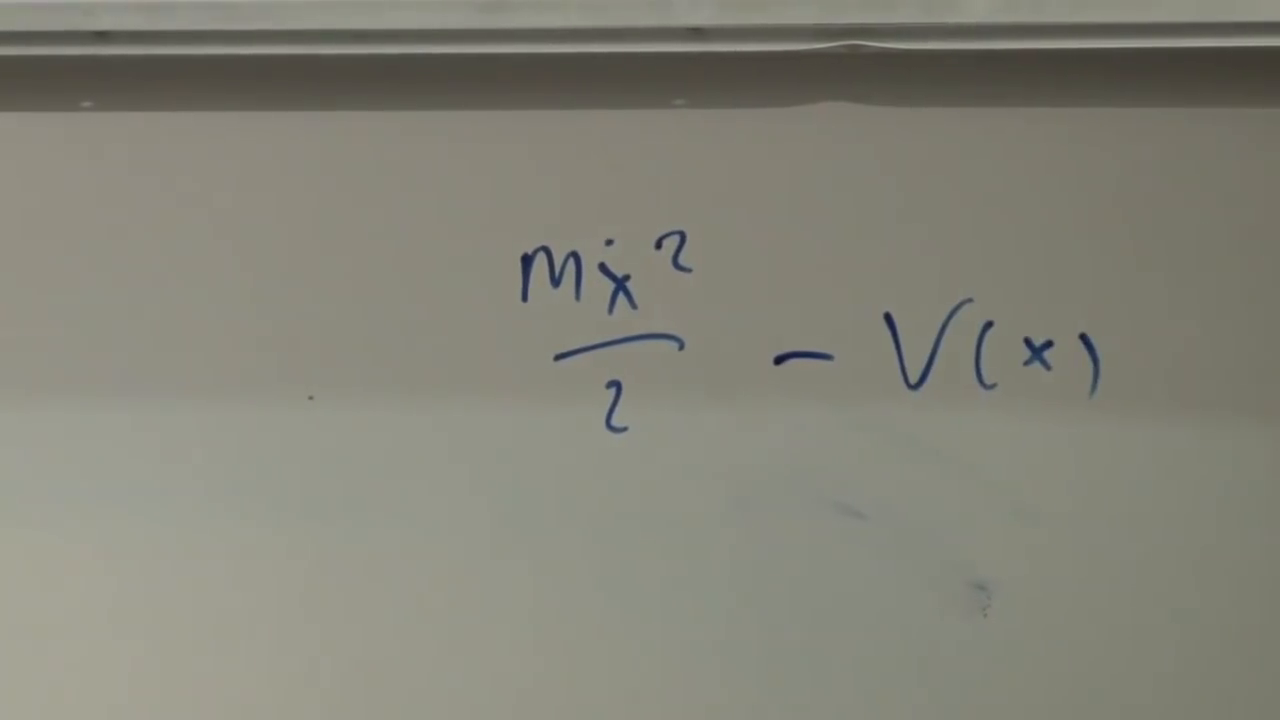
\includegraphics[width=0.72\textwidth]{lecture_04_figure_02.png}
  \caption{以動能減勢能的拉格朗日量說明共軛動量為\(m\dot x\)。}
  \lectureframe{00:14:48}
\end{figure}

如果\(q_i\)沒有出現在\(L\)中，那麼\(\dot p_i=0\)。這是利用循環座標導出守恆律的常見方法。兩者之間的真正關聯更為一般；先從例子中找出這種關聯，再加以證明，會更有幫助。

\section{尚未解釋便先找到的守恆定律}

\subsection{兩個座標與依賴間距的勢能}

令兩個質量都等於一，並取
\begin{equation}
  L=\frac{\dot q_1^{\,2}+\dot q_2^{\,2}}{2}-V(q_1-q_2).
  \label{eq:separation-lagrangian}
\end{equation}
可以想像兩個粒子在一條直線上運動。它們的交互作用只依賴彼此的間距。

\begin{figure}[htbp]
  \centering
  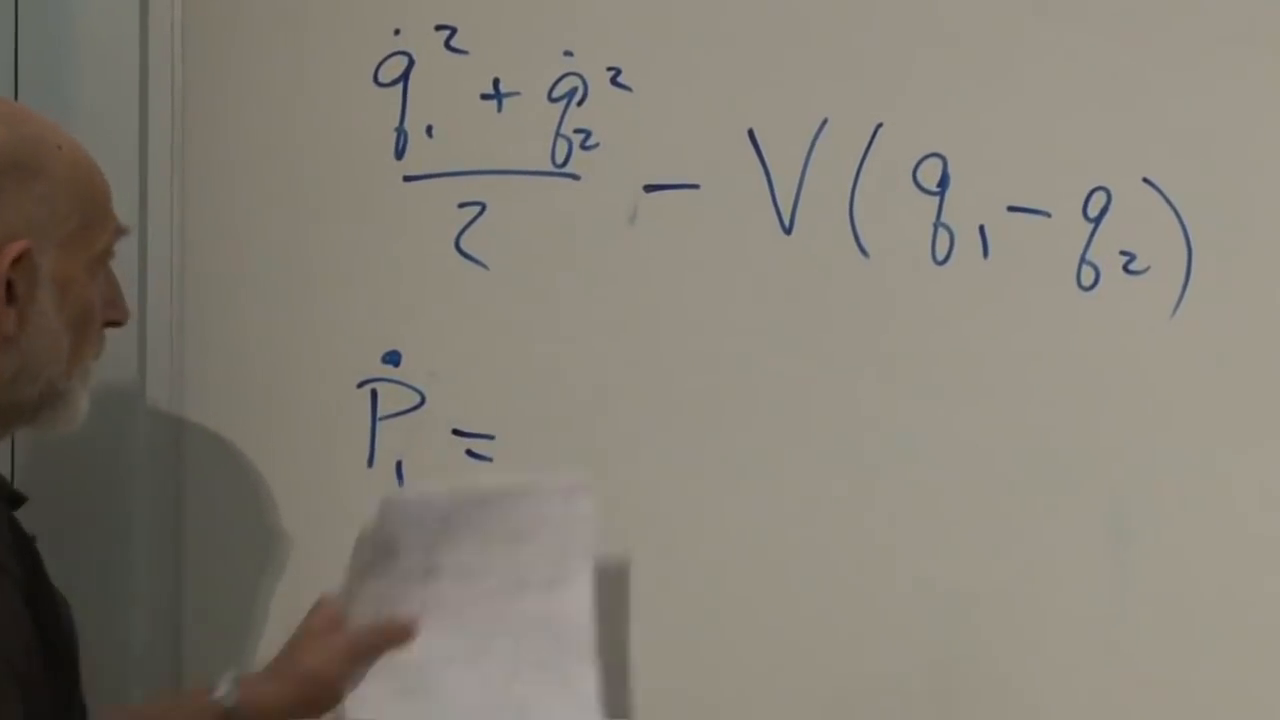
\includegraphics[width=0.78\textwidth]{lecture_04_figure_03.png}
  \caption{雙座標拉格朗日量，以及第一個動量方程的推導起點。}
  \lectureframe{00:18:56}
\end{figure}

以\(V'\)表示對\(V\)的自變數求導，
\begin{align}
  \dot p_1&=-V'(q_1-q_2),
  \notag\\
  \dot p_2&=+V'(q_1-q_2).
  \label{eq:separation-momentum-equations}
\end{align}
第二個方程的符號相反，因為增加\(q_2\)會使\(q_1-q_2\)減小。

\begin{classroomqa}
  \audiencequestion{第一個動量方程是否應該包含\(V'\)？負號從何而來？
  \lecturetimestamp{00:20:52--00:21:35}}
  \lecturerresponse{尤拉--拉格朗日方程表示
  \(\dot p_1=\partial L/\partial q_1\)，並不是說拉格朗日量等於零。由於\(L=T-V\)，對\(q_1\)微分會得到
  \(-V'\)。對\(q_2\)微分時，又因為\(q_1-q_2\)而多出一個負號，所以第二個方程中會出現\(+V'\)。}
\end{classroomqa}

\begin{figure}[htbp]
  \centering
  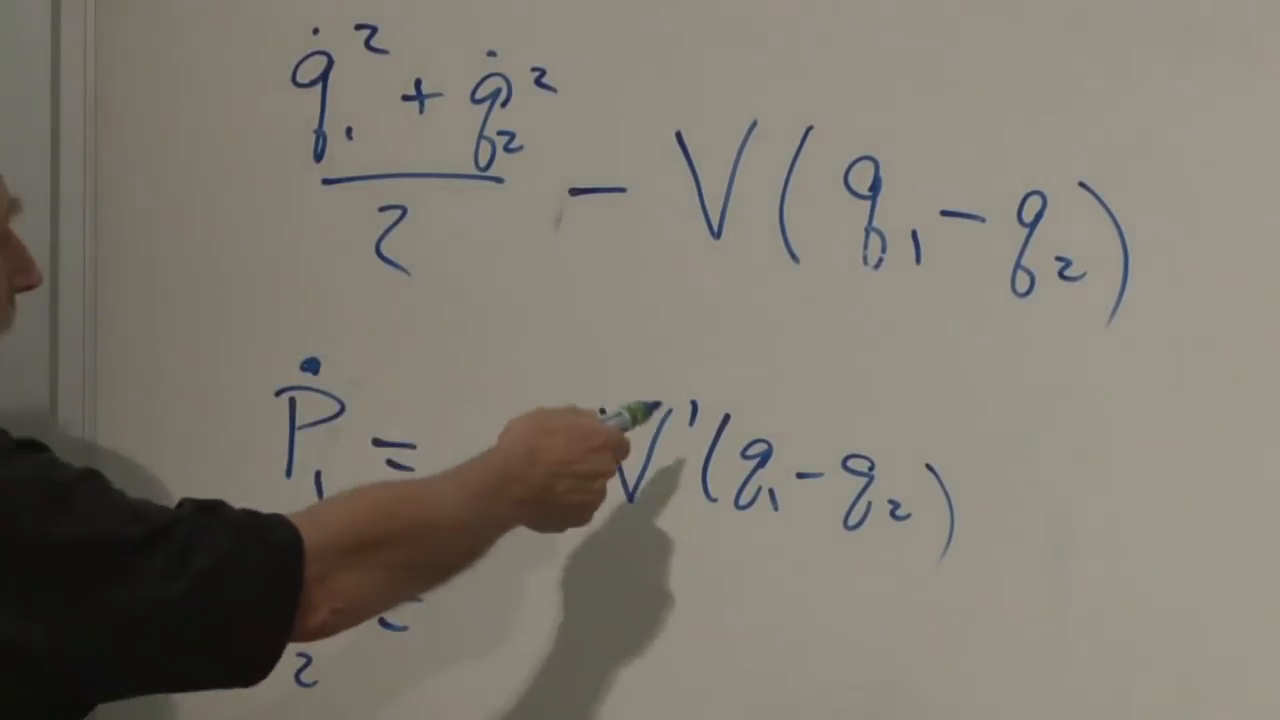
\includegraphics[width=0.78\textwidth]{lecture_04_figure_04.png}
  \caption{對\(p_1\)方程而言，導數的符號至關重要；\(p_2\)方程則有相反的符號。}
  \lectureframe{00:20:41}
\end{figure}

將式~\eqref{eq:separation-momentum-equations}相加，得到
\begin{equation}
  \frac{d}{dt}(p_1+p_2)=0.
  \label{eq:total-p-conserved}
\end{equation}
我們找到了守恆量，但還沒有解釋它為何存在。

\subsection{一個較不明顯的線性組合}

現在令
\begin{equation}
  L=\frac{\dot q_1^{\,2}+\dot q_2^{\,2}}{2}
    -V(Aq_1+Bq_2),
  \label{eq:ab-lagrangian}
\end{equation}
其中\(A\)和\(B\)是常數。於是
\begin{align}
  \dot p_1&=-A\,V'(Aq_1+Bq_2),
  \notag\\
  \dot p_2&=-B\,V'(Aq_1+Bq_2).
  \label{eq:ab-momentum-equations}
\end{align}
將第一個方程乘以\(B\)，第二個方程乘以\(A\)，再相減，就能消去力項：
\begin{equation}
  \frac{d}{dt}(Bp_1-Ap_2)=0.
  \label{eq:ab-conserved}
\end{equation}

\begin{figure}[htbp]
  \centering
  \includegraphics[width=0.78\textwidth]{lecture_04_figure_06.png}
  \caption{加權後的動量方程；力項在\(Bp_1-Ap_2\)中相消。}
  \lectureframe{00:24:20}
\end{figure}

\begin{classroomqa}
  \audiencequestion{從物理角度來看，像\(A\)和\(B\)這樣的常數可能從何而來？\lecturetimestamp{00:25:09--00:30:15}}
  \lecturerresponse{考慮兩個質量分別為\(m\)和\(M\)的粒子：
  \[
    L=\frac{m\dot X^2}{2}+\frac{M\dot Y^2}{2}-V(X-Y).
  \]
  重新定義尺度，使\(Q_1=\sqrt m\,X\)和\(Q_2=\sqrt M\,Y\)成立。動能項
  變為\((\dot Q_1^2+\dot Q_2^2)/2\)，而勢能則依賴於
  \(Q_1/\sqrt m-Q_2/\sqrt M\)。因此，不同的質量自然會成為線性組合中的係數。將\(Q_2\)換成\(-Q_2\)，會讓寫出的減號變成加號，而平方後的動能項不變。}
\end{classroomqa}

\begin{figure}[htbp]
  \centering
  \includegraphics[width=0.82\textwidth]{lecture_04_figure_07.png}
  \caption{質量加權座標使動能項更簡潔，同時將質量因子移入勢能。}
  \lectureframe{00:28:40}
\end{figure}

\begin{classroomqa}
  \audiencequestion{這是否表示，即使沒有循環座標，也可能存在守恆量？\lecturetimestamp{00:31:13--00:31:58}}
  \lecturerresponse{按目前寫出的變數來看，沒有\emph{明顯的}循環座標。變數變換或許能找出一個循環座標，但在這裡，尋找循環座標並不是有用的切入點。對稱性論證會直接找出守恆的組合。}
\end{classroomqa}

\section{對稱性的意義}

\subsection{平移}

先考慮質量為一的自由粒子，
\begin{equation}
  L=\frac{\dot q^2}{2}.
  \label{eq:free-unit-l4}
\end{equation}
將其運動歷程中的每一點都平移相同的常數：
\begin{equation}
  q'(t)=q(t)+\epsilon.
  \label{eq:free-translation}
\end{equation}
由於\(\epsilon\)與時間無關，\(\dot q'=\dot q\)，因此
\(\delta L=0\)。這種不變性就是平移對稱性。

有兩種等價的觀點。被動觀點是移動座標原點、物體則保持不動；主動觀點是固定座標軸、移動物體。採用主動的說法較不容易混淆：移動物理構型，看看\(L\)是否察覺。

對式~\eqref{eq:separation-lagrangian}而言，將兩個座標都平移：
\begin{equation}
  \delta q_1=\epsilon,
  \qquad
  \delta q_2=\epsilon.
  \label{eq:common-translation}
\end{equation}
速度不變，\(q_1-q_2\)也不變。

\begin{figure}[htbp]
  \centering
  \includegraphics[width=0.78\textwidth]{lecture_04_figure_08.png}
  \caption{共同平移不會改變兩個座標之間的距離。}
  \lectureframe{00:35:30}
\end{figure}

對式~\eqref{eq:ab-lagrangian}而言，採用較不明顯的變換
\begin{equation}
  \delta q_1=B\epsilon,
  \qquad
  \delta q_2=-A\epsilon.
  \label{eq:ab-transformation}
\end{equation}
速度同樣不變，而且
\begin{equation}
  \delta(Aq_1+Bq_2)=AB\epsilon-BA\epsilon=0.
  \label{eq:ab-invariant-argument}
\end{equation}
因此，這個變換是一種對稱性。

\begin{figure}[htbp]
  \centering
  \includegraphics[width=0.80\textwidth]{lecture_04_figure_09.png}
  \caption{保持\(Aq_1+Bq_2\)不變的非對稱平移。}
  \lectureframe{00:40:20}
\end{figure}

\begin{classroomqa}
  \audiencequestion{這些係數是否代表質量，使守恆量成為通常所說的質心動量？
  \lecturetimestamp{00:42:25--00:42:45}}
  \lecturerresponse{是。在質量加權變數中，對稱性和守恆量的組合看起來不對稱。換回\(X\)和\(Y\)後，就會得到通常的整體平移和總動量。}
\end{classroomqa}

\subsection{旋轉}

考慮平面中的單一粒子，
\begin{equation}
  L=\frac{m}{2}(\dot x^2+\dot y^2)-V(x^2+y^2).
  \label{eq:central-lagrangian-l4}
\end{equation}
這是中心力場的勢能。我們比較兩個彼此相對旋轉但各自固定的座標系；座標軸不會隨時間轉動。採用一致的旋轉方向，
\begin{align}
  x'&=x\cos\theta+y\sin\theta,
  \notag\\
  y'&=-x\sin\theta+y\cos\theta.
  \label{eq:finite-rotation-l4}
\end{align}

\begin{figure}[htbp]
  \centering
  \includegraphics[width=0.82\textwidth]{lecture_04_figure_10.png}
  \caption{中心力場的拉格朗日量，以及兩個經旋轉彼此對應的固定笛卡兒座標系。}
  \lectureframe{00:45:40}
\end{figure}

令\(\theta=\epsilon\)，並保留一階項：
\begin{equation}
  \cos\epsilon=1+O(\epsilon^2),
  \qquad
  \sin\epsilon=\epsilon+O(\epsilon^3).
  \label{eq:small-angle-l4}
\end{equation}
無窮小旋轉為
\begin{align}
  \delta x&=y\epsilon,
  &\delta y&=-x\epsilon,
  \notag\\
  \delta\dot x&=\dot y\epsilon,
  &\delta\dot y&=-\dot x\epsilon.
  \label{eq:infinitesimal-rotation-l4}
\end{align}

\begin{figure}[htbp]
  \centering
  \includegraphics[width=0.82\textwidth]{lecture_04_figure_11.png}
  \caption{座標和速度的無窮小旋轉。}
  \lectureframe{00:49:50}
\end{figure}

平移時，座標的改變量與原座標無關；旋轉則不同，\(x\)的改變量取決於\(y\)，而\(y\)的改變量取決於\(x\)。儘管如此，
\begin{align}
  \delta(x^2+y^2)
  &=2x\,\delta x+2y\,\delta y=0,
  \notag\\
  \delta(\dot x^2+\dot y^2)
  &=2\dot x\,\delta\dot x+2\dot y\,\delta\dot y=0.
  \label{eq:rotation-invariants-l4}
\end{align}
勢能項和動能項都保持不變。

\begin{figure}[htbp]
  \centering
  \includegraphics[width=0.76\textwidth]{lecture_04_figure_12.png}
  \caption{一階項相消，證明半徑平方在旋轉下不變。}
  \lectureframe{00:53:20}
\end{figure}

\section{一般守恆定理}

平移和旋轉這兩個例子有共同的形式。令一個連續的無窮小變換為
\begin{equation}
  \delta q_i=\epsilon f_i(q),
  \qquad
  \delta\dot q_i=\frac{d}{dt}\delta q_i,
  \label{eq:general-infinitesimal-symmetry}
\end{equation}
其中\(\epsilon\)與時間無關，而\(f_i\)可以依賴所有座標。

\begin{figure}[htbp]
  \centering
  \includegraphics[width=0.78\textwidth]{lecture_04_figure_13.png}
  \caption{一般的無窮小位移場
  \(\delta q_i=\epsilon f_i(q)\)。}
  \lectureframe{00:56:00}
\end{figure}

拉格朗日量的一階變分為
\begin{equation}
  \delta L
  =\sum_i\left(
    \frac{\partial L}{\partial q_i}\delta q_i
    +\frac{\partial L}{\partial\dot q_i}\delta\dot q_i
  \right).
  \label{eq:delta-l-general}
\end{equation}

\begin{figure}[htbp]
  \centering
  \includegraphics[width=0.84\textwidth]{lecture_04_figure_14.png}
  \caption{對\(\delta L\)的兩項貢獻：座標變分與速度變分。}
  \lectureframe{01:02:30}
\end{figure}

現在只考慮物理路徑，亦即尤拉--拉格朗日方程成立的路徑。利用
\begin{equation}
  \frac{\partial L}{\partial\dot q_i}=p_i,
  \qquad
  \frac{\partial L}{\partial q_i}=\dot p_i,
  \label{eq:el-substitution-l4}
\end{equation}
可得
\begin{align}
  \delta L
  &=\sum_i\left(\dot p_i\,\delta q_i
                +p_i\,\delta\dot q_i\right)
  \notag\\
  &=\frac{d}{dt}\sum_i p_i\delta q_i
  =\epsilon\frac{d}{dt}\sum_i p_i f_i(q).
  \label{eq:noether-derivation-l4}
\end{align}
關鍵步驟只用到乘法法則。

若此變換是對稱性，則\(\delta L=0\)。由於\(\epsilon\)是任意常數因子，
\begin{equation}
  \boxed{
  \frac{d\mathcal Q}{dt}=0,
  \qquad
  \mathcal Q=\sum_i p_i f_i(q)}
  .
  \label{eq:noether-charge-l4}
\end{equation}
這就是諾特定理在經典力學中的核心，適用於精確且不含時的點對稱性。

\begin{figure}[htbp]
  \centering
  \includegraphics[width=0.84\textwidth]{lecture_04_figure_15.png}
  \caption{利用乘法法則，從\(L\)的不變性導出守恆量。}
  \lectureframe{01:05:00}
\end{figure}

\begin{classroomqa}
  \audiencequestion{在\(f_i(q)\)中，\(q\)是否還有另一個指標？
  \lecturetimestamp{01:06:57--01:07:31}}
  \lecturerresponse{沒有指標的\(q\)代表整個集合\((q_1,q_2,\ldots)\)。每個分量\(f_i\)都可以依賴這些座標中的所有座標。例如，旋轉時\(f_x=y\)且\(f_y=-x\)。}
\end{classroomqa}

現在可以看出，這些例子並非偶然。共同平移有\(f_1=f_2=1\)，因此
\begin{equation}
  \mathcal Q=p_1+p_2.
  \label{eq:noether-common-p}
\end{equation}
非對稱平移有\(f_1=B\)和\(f_2=-A\)，因此
\begin{equation}
  \mathcal Q=Bp_1-Ap_2.
  \label{eq:noether-ab-p}
\end{equation}
旋轉時，\(f_x=y\)且\(f_y=-x\)：
\begin{equation}
  \mathcal Q=p_xy-p_yx.
  \label{eq:rotation-charge-sign}
\end{equation}
除旋轉方向的符號外，這就是角動量，
\begin{equation}
  J=xp_y-yp_x.
  \label{eq:angular-momentum-l4}
\end{equation}

\begin{figure}[htbp]
  \centering
  \includegraphics[width=0.82\textwidth]{lecture_04_figure_16.png}
  \caption{旋轉所對應的諾特荷，除方向符號外，等於平面上的角動量。}
  \lectureframe{01:11:00}
\end{figure}

對於多個彼此作用的粒子，將所有粒子一起旋轉。不變性所帶來的守恆量是它們的角動量總和，而不是每個粒子各自的角動量。

\section{關於定理適用條件的問題}

\begin{classroomqa}
  \audiencequestion{若座標軸旋轉，是否會使\(\delta L\)顯式地依賴時間？\lecturetimestamp{01:12:57--01:13:57}}
  \lecturerresponse{會。剛才的證明假設對稱性參數與時間無關，也就是固定的平移或固定的旋轉。參數隨時間變化的變換會產生額外項，需要更一般的處理。}
\end{classroomqa}

\begin{classroomqa}
  \audiencequestion{板書公式中的大寫\(Q\)是指變換本身嗎？\lecturetimestamp{01:14:02--01:15:58}}
  \lecturerresponse{不是。這個記號不巧與座標\(q_i\)相同。變換是\(\delta q_i=\epsilon f_i(q)\)；由此得到的守恆量是\(\mathcal Q=\sum_i p_i f_i\)。係數\(f_i\)表示第\(i\)個座標在對稱變換下如何改變。}
\end{classroomqa}

能量守恆也源於對稱性，但源自另一種對稱性：時間平移，也就是時間零點設在哪裡都不影響物理。這種情況以及哈密頓表述將留待後續討論。

\begin{classroomqa}
  \audiencequestion{能否透過改變座標系來吸收實際運動，讓力學只剩下座標變換？\lecturetimestamp{01:17:43--01:20:01}}
  \lecturerresponse{我們可以選擇一套座標來跟隨某個特定運動，但此時變換會依賴初始狀態和軌跡。此處使用的對稱變換則事先固定，不受系統採取哪個解的影響。表示運動本身時，在座標與動量組成的聯合空間中描述會更自然。}
\end{classroomqa}

\section{相空間中的諧振子}

令質量和彈簧常數都等於一，
\begin{equation}
  L=\frac{\dot q^2}{2}-\frac{q^2}{2}.
  \label{eq:oscillator-l4}
\end{equation}
由共軛動量和運動方程可得
\begin{equation}
  p=\dot q,
  \qquad
  \dot p=-q,
  \label{eq:oscillator-first-order-l4}
\end{equation}
也就是
\begin{equation}
  \dot q=p,
  \qquad
  \dot p=-q.
  \label{eq:oscillator-phase-flow}
\end{equation}
這些方程描述\(q\)-\(p\)平面上的等速圓周運動。在實空間中來回振盪的振子，是這個圓投影到\(q\)軸上的結果：在\(q=0\)處速率最大，在轉折點處則為零。

\begin{figure}[htbp]
  \centering
  \includegraphics[width=0.82\textwidth]{lecture_04_figure_17.png}
  \caption{諧振子的方程，以及它在\(q\)-\(p\)空間中的圓形軌道。}
  \lectureframe{01:25:30}
\end{figure}

\begin{classroomqa}
  \audiencequestion{相空間中的圓周運動是順時針方向嗎？
  \lecturetimestamp{01:25:47--01:27:15}}
  \lecturerresponse{是的，若將\(p\)軸置於水平方向、\(q\)軸置於垂直方向。在正\(q\)達到最大值時，\(\dot p=-q<0\)，因此運動方向朝下。若交換兩軸的位置，圖上看到的旋轉方向就會反過來；這也說明為什麼容易把座標慣例記錯。}
\end{classroomqa}

式~\eqref{eq:oscillator-phase-flow}中的這組方程已經很像哈密頓方程，但它完全是從拉格朗日力學推導出來的。

\section{連續對稱性與離散對稱性}

\begin{classroomqa}
  \audiencequestion{對稱性是否必須以無窮小的笛卡兒變換表示？\lecturetimestamp{01:27:48--01:30:31}}
  \lecturerresponse{笛卡兒座標只是方便的選擇；這項證明真正需要的是連續性。有些對稱性沒有無窮小版本。對偶勢而言，反射使\(q\mapsto -q\)且\(\dot q\mapsto-\dot q\)，但\(L\)保持不變；然而，反射無法由任意小的反射逐步組成。因此，這項經典推導不會為它導出相應的守恆量。}
\end{classroomqa}

\begin{figure}[htbp]
  \centering
  \includegraphics[width=0.82\textwidth]{lecture_04_figure_18.png}
  \caption{偶勢在離散反射\(q\mapsto -q\)下保持不變。}
  \lectureframe{01:29:30}
\end{figure}

\begin{classroomqa}
  \audiencequestion{如果守恆量\(\mathcal Q\)不等於零，是否表示該變換不是對稱性？
  \lecturetimestamp{01:30:40--01:31:30}}
  \lecturerresponse{不是。守恆量可以是任何常數值。應檢驗的是\(\dot{\mathcal Q}\)。若從某個假設的變換導出的量並不守恆，那麼在此證明的適用條件下，這個變換就不是對稱性。}
\end{classroomqa}

\begin{classroomqa}
  \audiencequestion{反射仍使拉格朗日量保持不變，為什麼它不能導出守恆律？\lecturetimestamp{01:31:34--01:32:27}}
  \lecturerresponse{不變性本身雖然看得出來，但推導過程還需要位移的一階變化，並用到乘法法則。反射以單一步驟，將位形空間的一側移到另一側。由於沒有無窮小生成元\(f_i\)，公式\(\mathcal Q=\sum_i p_i f_i\)就無從應用。}
\end{classroomqa}

\begin{classroomqa}
  \audiencequestion{由任意小的變換逐步構成的性質稱為什麼？\lecturetimestamp{01:32:36--01:33:23}}
  \lecturerresponse{這稱為\emph{連續對稱性}。平移和旋轉都是連續對稱性；反射則是\emph{離散對稱性}。}
\end{classroomqa}

\begin{classroomqa}
  \audiencequestion{如果許多無窮小步驟合成一個有限變換，被捨去的\(O(\epsilon^2)\)誤差會不會累積？\lecturetimestamp{01:33:23--01:36:10}}
  \lecturerresponse{無窮小不變性必須在變換過程中到達的每一點都成立，而不只是起點。將有限的參數區間分成\(N\)步，每步大小為\(\epsilon\)：累積的一階位移為\(N\epsilon\)，而局部的\(O(\epsilon^2)\)餘項累積為\(N\epsilon^2=(N\epsilon)\epsilon\to0\)。這就是連續變換群所形式化的局部到有限變換的過程。}
\end{classroomqa}

\begin{classroomqa}
  \audiencequestion{離散對稱性會在經典系統中實際出現嗎？\lecturetimestamp{01:36:32--01:37:25}}
  \lecturerresponse{當然會。諧振子本身就具有偶勢\(V(q)\propto q^2\)，因此在\(q\mapsto -q\)下保持不變。這類例子很多；這裡要指出的只是，這種離散不變性不會提供新的經典諾特荷。}
\end{classroomqa}

\begin{classroomqa}
  \audiencequestion{可是，連續和離散變換都使\(L\)保持不變，這不就是同一個條件嗎？\lecturetimestamp{01:37:37--01:39:18}}
  \lecturerresponse{就不變性而言，兩者都是對有限變換的陳述；但它們不是這項證明所需的同一種數學條件。證明需要一階變分。對反射而言，「一階」沒有意義，因此導出守恆荷的推導根本無法開始。}
\end{classroomqa}

\begin{classroomqa}
  \audiencequestion{從歷史角度來看，這與諾特定理有何關聯？\lecturetimestamp{01:39:26--01:40:42}}
  \lecturerresponse{這只是艾美・諾特更一般定理中的一個受限部分。對稱性與守恆量之間的某些特定關聯早已為人所知，但諾特在二十世紀初將它們納入統一且極為一般的架構中。學界並未公平對待她在數學上的重要貢獻。}
\end{classroomqa}

\begin{classroomqa}
  \audiencequestion{經典力學仍是活躍的研究領域嗎？\lecturetimestamp{01:40:47--01:42:37}}
  \lecturerresponse{是。這裡用到的初等定理由來已久，但非線性動力學、可積系統、混沌、流體和幾何力學仍是內容豐富的研究領域。對稱性原理的適用範圍也遠超過經典粒子力學。}
\end{classroomqa}

\section{作用量原理為何重要}

\begin{classroomqa}
  \audiencequestion{對稱性蘊含守恆，有沒有直觀的理由？\lecturetimestamp{01:42:49--01:47:57}}
  \lecturerresponse{光有對稱性還不足以說明這一點。考慮黏滯阻力，
  \[
    m\ddot x=-c\dot x.
  \]
  此方程在\(x\mapsto x+\epsilon\)下保持不變，但當\(p=m\dot x\)時，
  \[
    \dot p=-\frac{c}{m}p,
    \qquad
    p(t)=p(0)e^{-ct/m},
  \]
  動量仍會衰減。這是描述子系統的有效方程，並不是只針對\(x\)的基本作用量駐值定律。若將流體分子和封閉系統的其餘部分也納入，總動量便會守恆。對稱性與守恆之所以相連，是透過拉格朗日作用量原理，而不是只因為方程呈現某種形式的微分方程。}
\end{classroomqa}

\begin{figure}[htbp]
  \centering
  \includegraphics[width=0.65\textwidth]{lecture_04_figure_19.png}
  \caption{平移不變的黏滯阻力，然而約化後的粒子動量仍會衰減。}
  \lectureframe{01:44:30}
\end{figure}

\begin{classroomqa}
  \audiencequestion{能否定量說明，物理路徑何時不是作用量的極小值？\lecturetimestamp{01:48:08--01:51:38}}
  \lecturerresponse{真正的極小值很罕見；作用量在路徑空間中通常呈鞍點形狀。對質量和彈簧常數皆為一的振子而言，
  \[
    S[q]=\frac12\int(\dot q^2-q^2)\,dt.
  \]
  狹窄且快速變化的形變會增加正的\(\dot q^2\)項。若形變較寬廣，並在長時間內維持些微偏移，負的\(-q^2\)項便可能占上風，使作用量降低。因此，同一條駐值路徑既有使作用量增加的方向，也有使其降低的方向。量子力學透過路徑積分的觀點，給出了駐值條件更深層的起源；這項論證將留待後續討論。}
\end{classroomqa}

\begin{figure}[htbp]
  \centering
  \includegraphics[width=0.80\textwidth]{lecture_04_figure_20.png}
  \caption{一條較寬廣的鄰近振子路徑，說明作用量駐值通常呈鞍點而非極小值。}
  \lectureframe{01:50:20}
\end{figure}

\begin{classroomqa}
  \audiencequestion{連續對稱性與守恆律是否一一對應？\lecturetimestamp{01:51:44--01:52:43}}
  \lecturerresponse{在變分框架內，並且排除等價或平凡的情況後，基本上可以這樣理解。每個連續對稱性都有一個守恆荷，而守恆量通常也能追溯到某種對稱性。精確表述帶有技術上的限定條件，因此不應輕率套用這種概括說法。}
\end{classroomqa}

\begin{classroomqa}
  \audiencequestion{每個拉格朗日量都必須具有非平凡的對稱性嗎？\lecturetimestamp{01:52:43--01:53:23}}
  \lecturerresponse{不必。這裡舉的例子刻意選擇了具有對稱性的系統。一般的拉格朗日量不見得在任何假設的空間變換下保持不變。}
\end{classroomqa}

\begin{classroomqa}
  \audiencequestion{最後，對稱性應該理解為主動運動，還是被動座標變換？\lecturetimestamp{01:53:25--01:55:08}}
  \lecturerresponse{兩種描述都可以彼此等價，但在這裡主動描述較為簡潔。移動整個物理系統，並觀察拉格朗日量是否改變。若採用被動描述，則必須說明：座標架移動時，拉格朗日量的\emph{形式}保持不變。}
\end{classroomqa}

\begin{classroomqa}
  \audiencequestion{接下來要談什麼？\lecturetimestamp{01:55:10--01:55:35}}
  \lecturerresponse{接著將討論能量守恆、它與時間平移對稱性的關聯，以及哈密頓表述。}
\end{classroomqa}
